% uncommented header -> document does not compile if that is still included (R. Nawrodt)

%\documentclass[11pt,a4paper]{article}
%\usepackage{verbatim}
%\usepackage[latin1]{inputenc}
%\usepackage[T1]{fontenc}
%\usepackage{ae}
%\usepackage{color}
%\usepackage{parskip}
%\usepackage{xspace}
%\usepackage[english]{babel}
%\usepackage{thumbpdf}
%\usepackage[pdftex,a4paper,pagebackref=true,pdfpagelabels=true]{hyperref}
%\definecolor{linkcolor}{rgb}{.8,0,0}
%\definecolor{urlcolor}{rgb}{0,0,.7}
%\definecolor{citecolor}{rgb}{0,.5,0}
%\definecolor{acrocolor}{rgb}{0,0,.7}
%\hypersetup{bookmarksopen,colorlinks=true}
%\hypersetup{pdfstartview=FitH}
%\hypersetup{linktocpage=true,bookmarksnumbered=true}
%\hypersetup{plainpages=false,breaklinks=true}
%\hypersetup{linkcolor=linkcolor,citecolor=citecolor,urlcolor=urlcolor}
%\usepackage{float}
%\usepackage{tabularx}
%\usepackage[pdftex]{graphicx}
%\usepackage{epstopdf}

%\usepackage{url}



%\title{ Vacuum Systems}
%\author{C. Bradaschia, G. Parguez, A. Pasqualetti\\ European Gravitational Observatory}

%\begin{document}
\FloatBarrier
\subsubsection{Vacuum Systems}


\paragraph{Introduction}  \label{intro}

In laser interferometers for GW detection most of the instrument has to be kept under High-Vacuum or Ultra-High-Vacuum (HV, UHV) for several reasons:
\begin{itemize}
\item reduce the noise due to vacuum fluctuations along the beam path to an acceptable level
\item isolate test masses and other optical elements from acoustic noise
\item reduce test mass motion excitation due to residual gas fluctuations
\item reduce friction losses in the mirror suspensions
\item contribute to thermal isolation of test masses and of their support structures
\item contribute to preserve the cleanliness of optical elements.
\end{itemize}


A vacuum system of this kind (Fig.~\ref{fig:vac1}) is composed of several UHV pipes with kilometric length and several cylindrical vertical HV/UHV tanks (towers) containing the optical elements and their support structures (Fig.~\ref{fig:vac2}). In general it is necessary to have the whole vacuum system constituting one single volume, without physical separations (windows) on the laser beam path. HV volumes (the towers) contain parts of the apparatus not easily compatible with UHV pipes where, on the contrary, the large majority of the laser beam has to travel. The separation between HV and UHV is obtained by differential pumping or by cryogenic traps, stopping the migration of water and other high vapor pressure components.

\begin{figure}
\begin{center}
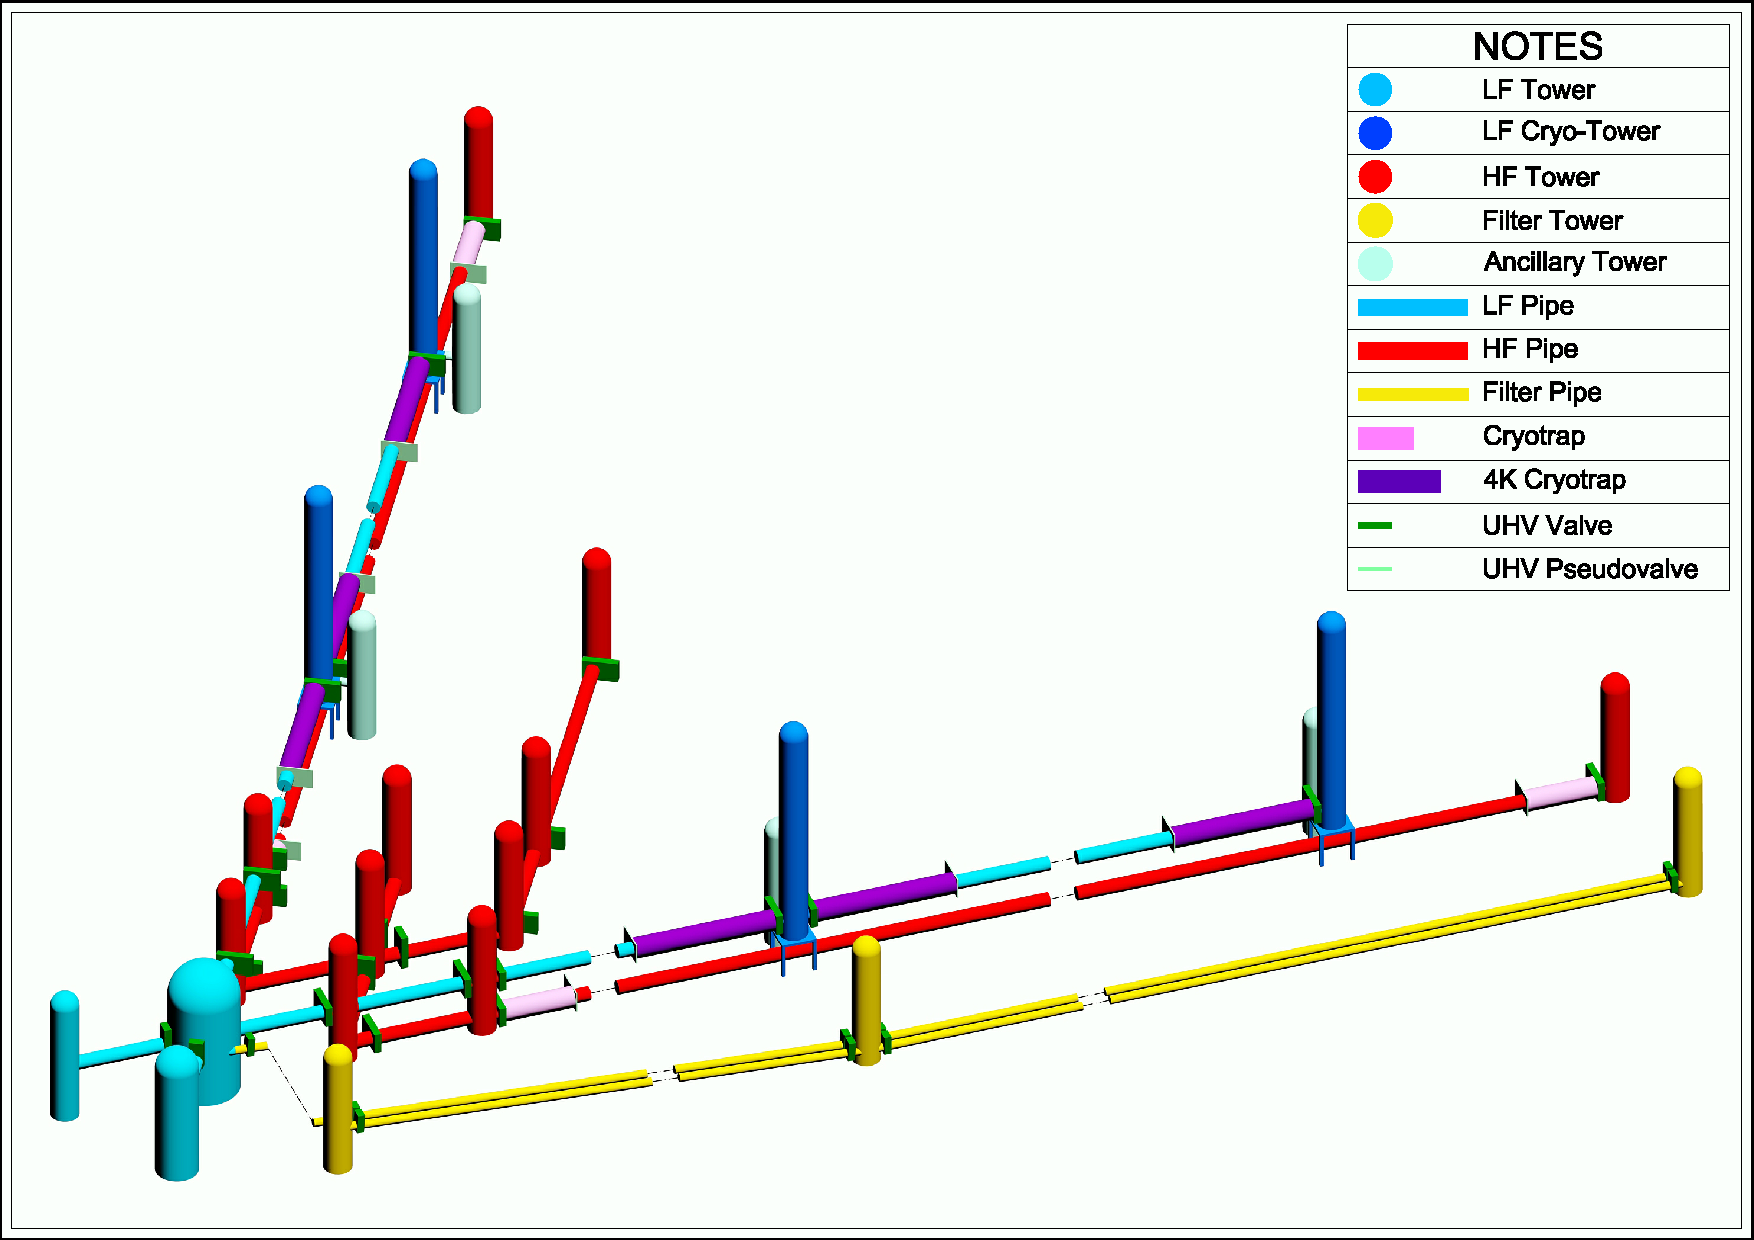
\includegraphics[width=\textwidth]{Sec_SiteInfra/Figures/VAC1.pdf}
\caption{Schematic of the ET vacuum system lay-out, out of scale. Only one xylophone detector is shown, out of three.}
\label{fig:vac1}
\end{center}
\end{figure}

\begin{figure}
\begin{center}
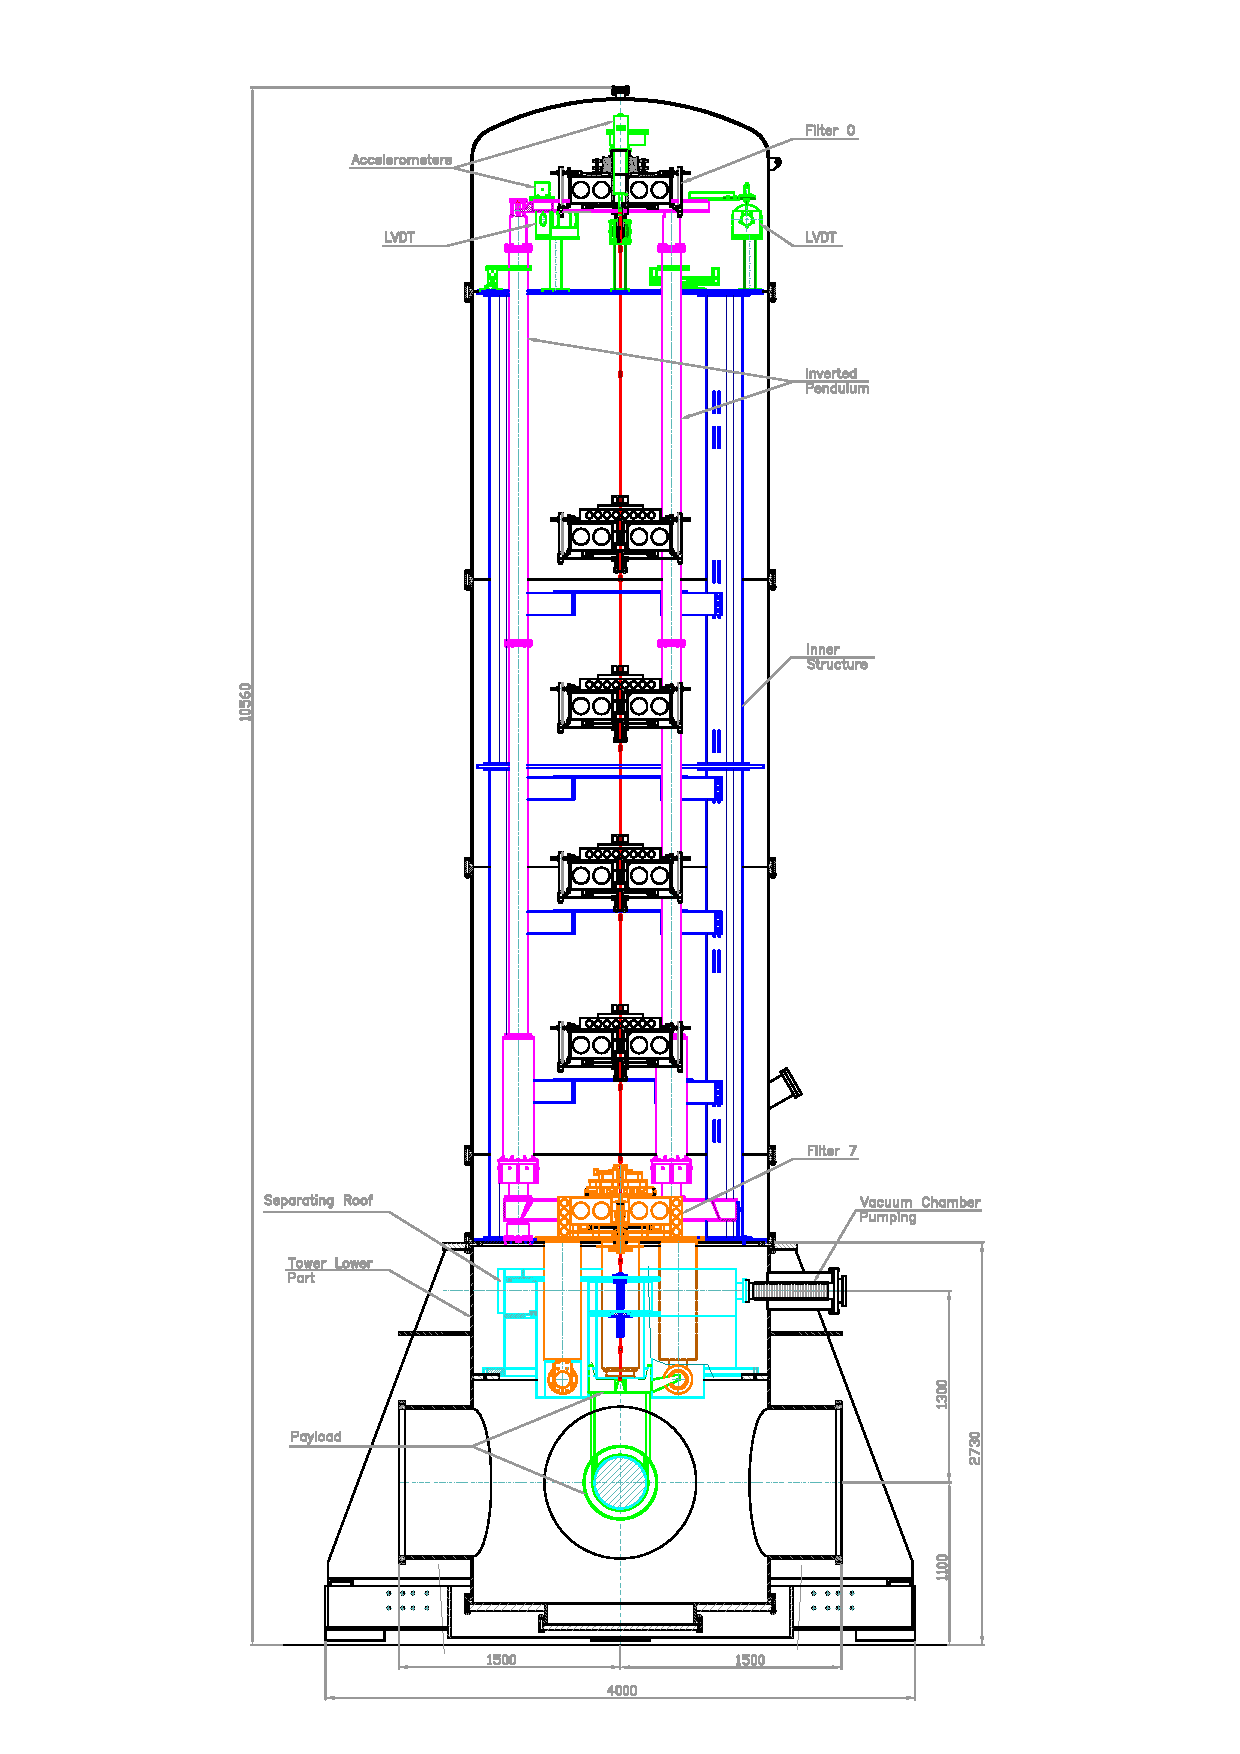
\includegraphics[width=\textwidth]{Sec_SiteInfra/Figures/VAC2.pdf}
\caption{As an example the cross-section of a Virgo a mirror tower is shown.}
\label{fig:vac2}
\end{center}
\end{figure}


The vacuum enclosure will be built of stainless steel (304L); this material is preferred for its easy availability, its price, the large experience in machining and welding, the mechanical properties (ductility), the chemical properties and the achievable outgassing rate. The same choice has been made in the past for Virgo, LIGO, GEO600.



\paragraph{Average base pressure in the arm pipes} \label{average_pressure}

The noise due to vacuum fluctuations (index instabilities due to statistical fluctuations of the number of molecules in the volume occupied by the laser beam in the arms cavities) has been calculated by several people for Virgo and LIGO \cite{cella08}. It is (at first approximation) inversely proportional to the square root of the beam volume (or to the square root of the beam average radius or to the square root of the arm length or to the square root of the average pressure).
The following baseline parameters have been used:
\begin{itemize}
\item arm length:  					10 km
\item beam waist:  					40 mm (TEM00) @ 5 km
\item beam average radius on mirrors: 		120 mm
\item best sensitivity:  				$\sim 3\,10^{-25}$\,Hz$^{-1/2}$ @ 300\,Hz.
\end{itemize}


As it is common practice in matter of vacuum, we will take a safety factor of at least $10$ with respect to the pressure producing a phase noise at the limit of the best sensitivity. The residual gas composition will be dominated by hydrogen with presence of water and other gases; we will aim to keep the residual pressure at level of $1\,10^{-10}$\,mbar (H$_2$ and H$_2$O, each at $5\,10^{-10}$ mbar, would generate an overall noise level of about $2\,10^{-25}$ Hz$^{-1/2}$, see Fig.~\ref{fig:vac3}). The vacuum system will be extremely clean from heavy organic molecules, both to limit the phase noise and to prevent pollution of the optical components. Hydrocarbon partial pressure shall be at the level of $10^{-14}$ mbar.

\begin{figure}
\begin{center}
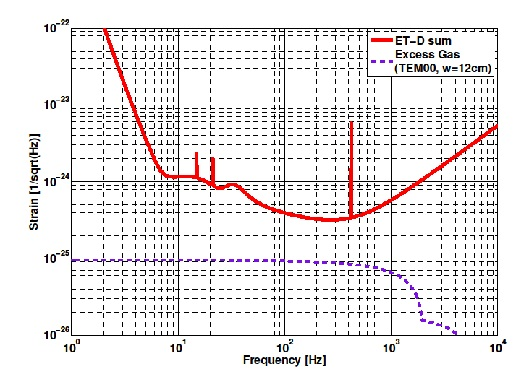
\includegraphics{Sec_SiteInfra/Figures/VAC3.jpg}
\caption{Phase noise given by selected gases compared to the expected sensitivity, computed for the appropriate beam profile. (Gas composition: Hydrogen [$1\,10^{-10}$ mbar], Water [$5\,10^{-11}$ mbar], Nitrogen [$1\,10^{-11}$ mbar])}
\label{fig:vac3}
\end{center}
\end{figure}


To reach these conditions it will be necessary:

\begin{itemize}
\item to fire (one week in an air oven at 450$^\circ$C) the stainless steel vacuum enclosure elements (or the raw material sheets) in order to reduce the H$_2$ outgassing rate at the level of $10^{-14}$ mbar l /cm$^{2}$ s
\item to bake for one week at $150^\circ$C the pipes already assembled and under vacuum in order to eliminate the water molecule layers sticking to the pipe inner wall.
\end{itemize}


Liquid nitrogen cryotraps will be necessary to separate the baked UHV pipes from the water dominated unbaked mirror towers, in HV regime. Concerning the phase noise, the path length of the beams in HV will be kept short, that is a negligible noise contribution, when compared to the kilometers in the UHV arm pipes.
Large gate valves will be put at each end of the arm pipes, in order to preserve vacuum when venting a tower. For the same reason each tower will be separable from the rest of the vacuum enclosure by suitable gate valves.
The reference cavities being less sensitive to vacuum noise require a residual pressure at the level of $10^{-7}$ mbar. Their pipes will not be fired at 450$^\circ$C nor baked at 150$^\circ$C.

\paragraph{The arm pipes}

Due to the multi interferometer/xylophone choice for ET, several beams will run along each side of the triangular tunnel, we assume four main beams and two filter cavity beams, taking into account all the three detectors (six interferometers) composing the full ET.

The chosen baseline configuration includes four pipes, one for each main beam: two with a $0.9$ m diameter for the HF interferometers and two $0.75$ m diameter pipes, for the LF interferometers. In addition, two $0.69$ m pipes for the two filter cavity beams belonging to each LF interferometer. HF interferometers will be equipped also with a 700 m long filter cavity, running in a dedicated tunnel, inside a 0.6 m diameter pipe.

The pipes will be arranged inside the tunnel cross-section as shown in Fig.~\ref{fig:vac4}: the filter cavities at the bottom, under a movable floor, the two HF beams on the floor at the tunnel sides and the two LF beams on top of them (see below the "Tower" paragraph).

\begin{figure}
\begin{center}
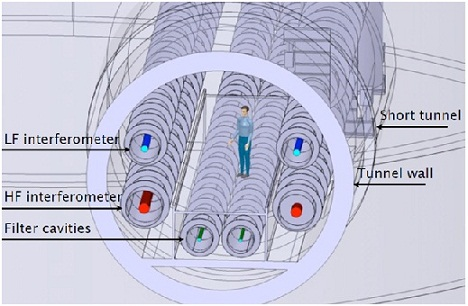
\includegraphics{Sec_SiteInfra/Figures/VAC4.jpg}
\caption{Arrangement of the vacuum pipes in the tunnel cross-section.}
\label{fig:vac4}
\end{center}
\end{figure}

The pipe construction procedure merges Virgo and LIGO experience, even if the final choice will be performed in due time, with the appointed company. The pipes will have thin walls (3 -- 4 mm) with external stiffening rings, every 1 -- 2 meters. Two ring s will be larger, serving as attachment for the supports (see below).

20 m long pipe elements will be fabricated by continuous spiral welding in a suitable clean factory installed on site. At one end of each element a suitable bellows will be added to accommodate thermal expansion, during bake-out; winter/summer temperature excursion should be negligible under ground. At both ends 2 mm thick lips will be added, to allow UHV compatible welding of adjacent elements, without inert gas protection on the inner side of the weld (this technique has been successfully applied in Virgo).

Simple supports ``a la LIGO'', using steel cables and adjustable stretching screws will be sufficient, coping with the relatively high stability of an under ground tunnel.

The pipes will be aligned in the tunnel using optical instruments and laser beams, since GPS will not be applicable under ground. The requested straightness error for the arms is of the order of 10 mm. Periodical surveys will be necessary every few years, in order to detect dangerous pipe displacements due to ground movements.

Each 10 km pipe will contain a few hundreds of metallic baffles for diffused light mitigation. They shall be made out of stainless steel with a suitable conical shape and serrated inner edge (Fig.~\ref{fig:vac5}) against diffraction. The radial width of the baffles, between 50 and 100 mm, and their position will be determined by a suitable simulation~\cite{vinet97,vinet96}.

\begin{figure}
\begin{center}
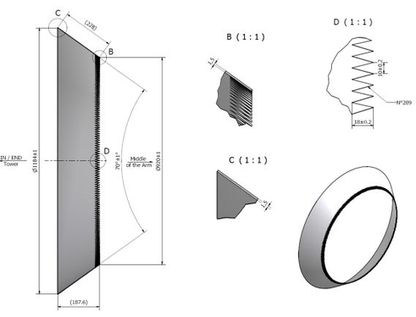
\includegraphics{Sec_SiteInfra/Figures/VAC5.jpg}
\caption{As an example the Virgo pipe conical baffles are shown.}
\label{fig:vac5}
\end{center}
\end{figure}


\paragraph{Pipe Assembly}

The $20$ m pipe elements will be lowered to the corner caverns with the ends sealed by suitable end-caps and equipped with thermal insulation; each element will weight about $1.5$ t. The element will be put on and bolted to a simple carriage made of two parallel $20$ m long beams supported by small train wheels. In this way pipe elements can be pushed to their position one after the other by an electric tractor running on $5$ km long rails reaching up to mid arm. The rails, two for each pipe, are supported by frames extending to the whole tunnel cross-section. These same frames have the function, as said before, of supporting the pipes.
In alternative the element could be suspended to a $20$ m long beam running, as a bridge crane carriage, attached to a $5$ km long rail. The rail, one per pipe, is supported by the already mentioned frames. Also in this case pipe elements can be pushed to their position one after the other by an electric tractor or by a traction line.

Every $500$ m, along the tunnel, there is an enlarged room to accept pumping, bake-out and control equipment; those rooms are used also to weld the pipe elements at ease in a wide area, under a clean tent.

The first pipe element is stopped with the rear end under the tent; when the front end of the second element is close, the sealing lids are removed, after starting appropriate clean air flows. The corresponding end lips of the adjacent elements are precisely adjusted and welded. The beams of the two carriages (under or above the pipe, according to the chosen option) are rigidly bolted together, taking care of appropriate compression/extension of the bellows.

The two modules are shifted forward until the rear end of the second module is at the welding position; now the front end of the third module is adjusted and welded as before. This procedure is continued until the $25^{th}$ module is welded and the $500$ m long section of pipe is completed.

The ends of the assembled pipe section are closed with vacuum tight lids, the section is evacuated and tightness tests are performed. The closing lids will be strongly fastened to the tunnel wall, in order to keep the $6.4$ t axial load due to atmospheric pressure.

The $500$ m long section will be then vented and shifted by $20$ m to its final position.

Every pair of upper support cables (as said, in the LIGO style) are attached to the corresponding support ring, the cables are tightened, the bolts of the pipe elements to the carriages are removed, the elements are lifted (lowered, in the case of suspended transportation) by $10$ mm in $1$ mm steps. The $500$ m long train composed by $25$ carriages is sent back to the end cavern, to start the assembly of the second $500$ m pipe section. The lower support cables are attached to the support rings and suitably tightened.

The clean tent and the welding equipment are transferred to the next enlarged room and the assembly of the second $500$ m pipe section is started. Once completed and vacuum tested, taking advantage of the bellows and of the support cables, the front lip of the new 500\,m section is adjusted to the rear lip of the previous section and welded. This final weld is the last to be performed in that particular enlarged room.

The procedure continues contemporarily extending the installed pipe from mid arm to both arm ends.

Concerning the pipes arrangement in the tunnel, it is necessary to have the possibility to inspect and repair the welds between pipe elements. This could be achieved leaving a clearance of about 0.5\,m between the ``nude'' pipes and the tunnel wall (at least every 20\,m). We should consider also the case of needs of (small) maintenance interventions on the tunnel wall lining.

A pumping station room is sketched in Fig.~\ref{fig:VAC7}. In practice it is an enlargement of the tunnel for a width of 12\,m and a length of 10\,m, allowing the installation of the pumps, which are hold in their position by a metallic frame not reported in the sketch. Three cabinets  housing the electronics of the vacuum equipment are included, together with an electrical power supply for baking (60\,VDC 300\,kW).

A bridge crane shall be present, and the room shall probably need a conditioned humidity and temperature, to allow electronics efficiency.

\begin{figure}
\begin{center}
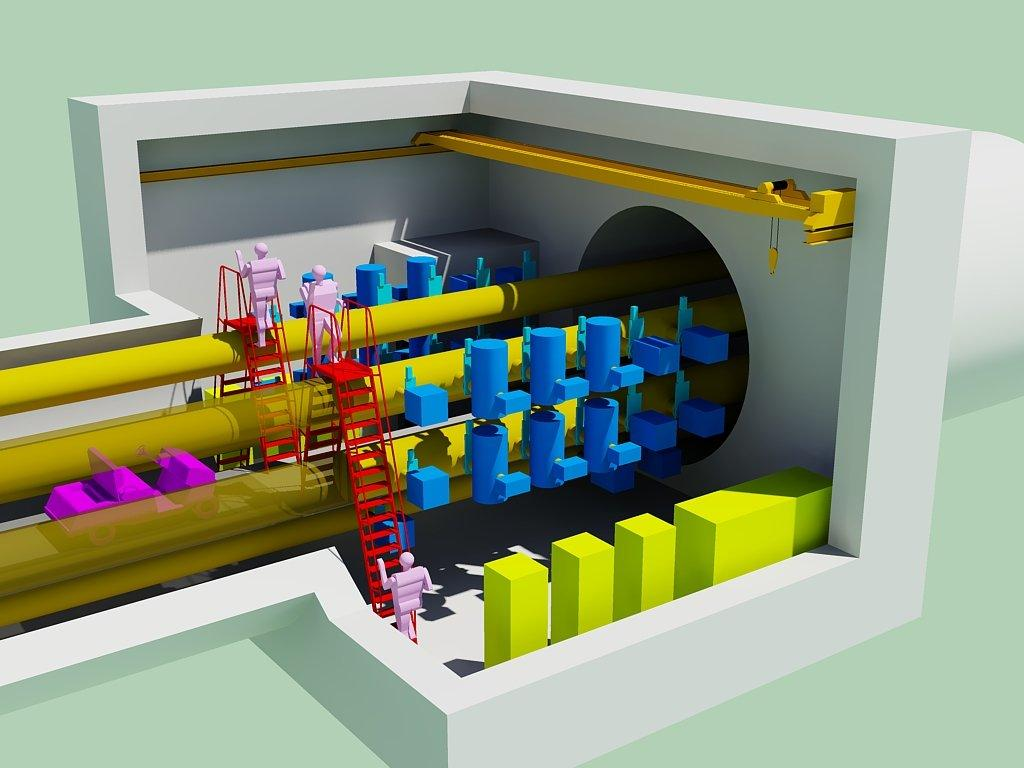
\includegraphics[width=\textwidth]{Sec_SiteInfra/Figures/VAC7.jpg}
\caption{3D view of a pumping station: the blue objects represent the pumps and sensors, the yellow ones the cabinets for pumps control (1 per tube) and baking power supply (1 cabinet for all). A separate small room is reserved for the high voltage electrical transformer.}
\label{fig:VAC7}
\end{center}
\end{figure}


\paragraph{Pipe pumping system}

The pipe pumping system has been conceived to be composed of standard modules, grouped together, in order to limit the number of pumping stations along the arms.

The goal total residual pressure (hydrogen and other gases) of $1\,10^{-10}$ mbar can be obtained, after firing and bake-out (see a previous paragraph), with one 5000 l/s pumping group, every 500 m, both in a 0.9 m and in a 0.7 m diameter  pipe, the smaller gas load due to the smaller diameter being compensated by the relatively reduced conductance.

Below is described the pumping system for one single pipe. 

Each permanent pumping group will consist of three identical modules, each made of one 2500 l/s Ti sublimation pump (TSP), connected to the pipe through a 250 mm gate valve (the Ti will be sublimated not in the tube but in a separated chamber), coupled to a 300 l/s ion pump. The former to pump active gases, the latter to pump inert gases. At such a low pressure TSPs are expected to require not more than one yearly regeneration. NEG pumps are being considered as a possible alternative to TSPs. Some redundancy is necessary to cover the Ti pumps regeneration periods.

Besides the permanent pumping group, every pumping station will include suitable vacuum gauges and two 2000 l/s turbo, backed by a scroll pump, for initial evacuation and bake-out.

The Filter cavity pipes, requiring a $10^{-7}$ mbar residual pressure, will be equipped only with the turbo/scroll groups, possibly reinforced with $77$ K cryo-pumps.

Every 10 km pipe will have three RGA's, at each end and in the middle, to monitor the vacuum quality and for easier diagnosis in case of problems.

\paragraph{Pipe bake-out system}

In order to perform the 10 days bake-out under vacuum at 150$^{\circ}$C, the pipe could be heated by electrical current flowing in its walls, closing the circuit by a suitable Al bar or cable. Closing the circuit with the pipe of the adjacent twin interferometer would save the Al conductor cost, but does not seem practical. The use of DC will assure a uniform current and temperature distribution on the pipe walls and improve human safety. Typical arrangement of the circuit could be, similar to Virgo, a series of double ring circuits with one DC source every 500 m delivering 1000 A at 50 V along 250 m in each direction. Such a system will deliver 200 W per meter of pipe, which has been experimentally demonstrated to be sufficient to reach 150$^{\circ}$C, if the pipe is wrapped in a suitable 10-20 cm thick thermal insulation layer. Each DC source will consist of a transformer/rectifier supplied by medium voltage AC (15 kV). This choice is dictated to reduce the cross section of cables to distribute 2 MW along 10 km. 15 kV equipment will be confined in dedicated rooms.

In this configuration, delivering 300 W per meter of tunnel, in absence of ventilation, a very crude estimate considering a 6 m aperture tunnel, drilled in isotropic rocks (assumed  $\rho = 2500$ kg/m$^{3}$, k = 2.0 watt/m K, C = 800 joule/kg K) gives an increase of room and wall temperature by about +13$^{\circ}$C after a 10 days bake-out. This situation, being at the limit of what could be tolerable, suggests to exploit several remedies like baking at a lower temperature for more days and improving the thermal insulation properties, in order to reduce the temperature increase of the tunnel walls. A suitable air cooling system will be designed to reduce further the ambient temperature (possibly renewing once per hour the tunnel air volume). The overall power release inside the tunnel could be reduced also performing bake-out in sequence on shorter pipe sections, separated by ``pseudo-valves'', vacuum tight, but able to sustain null pressure difference.

\paragraph{Cryotraps}

As stated above, HV volumes (e.g.\ the towers) will communicate with the UHV pipe through liquid nitrogen cryotraps, to prevent migration of water and other high vapor pressure contaminants. In order to allow the beam passage the cryotraps will consist of a large hollow muff, containing liquid nitrogen, suspended inside an increased diameter pipe section, with a design very similar to the one adopted for LIGO, Virgo and Advanced Virgo (Fig.~\ref{fig:vac6}). The lateral surface will be thermally isolated by a few cylindrical metal screens; the heat exchange at both ends will be limited by suitable circular baffles, leaving passage for the beam. The propagation of mechanical noise due to liquid nitrogen bubbling will be limited installing cryotraps at least 20 m away from the mirror towers; this will help to avoid excessive cooling of the mirrors (to avoid condensation, in no circumstance a mirror should be the coldest point in the environment). Cryotraps will have valves at each end, in order to be confined during warming-up for regeneration (not more than once per year). The traps will be 7--10 m long for pipes with diameters of 0.6--1.0\,m. The liquid nitrogen consumption has been evaluated to be about 10 liters per hour per trap. In correspondence of the cryogenic towers for the 4 K mirrors of the LF interferometer, the cryotraps will be much longer (50\,m) and will include liquid helium sections to strongly limit the mirror heat exchange as described in the following section. We refer to the same section for a description of the supply plant for cryogenic liquids.

\begin{figure}
\begin{center}
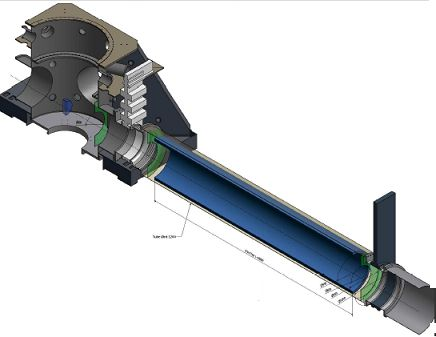
\includegraphics{Sec_SiteInfra/Figures/VAC6.jpg}
\caption{A liquid nitrogen cryotrap.}
\label{fig:vac6}
\end{center}
\end{figure}

\paragraph{Towers}

Mirror towers upper part will have a 2--3\,m diameter to contain easily the pendulum chains of Superattenuators and the inverted pendulum legs; the structure will be an evolution of the Virgo towers~(Fig. \ref{fig:vac2}). The lower chamber of the towers will have a diameter up to 3\,m, to contain large payloads. The HF interferometer towers will have a large bottom lid to allow installation of payloads from a clean basement, under a filtered air shower. The height will be 10 m for the main mirrors of the warm HF interferometer. Auxiliary mirrors or benches requiring lower isolation, will be located in shorter towers. The towers containing the cryogenic mirrors of the LF interferometer, to achieve full seismic isolation performance down to 2\,Hz, will be up to 20\,m tall. In these towers, sitting on top of the HF interferometer, the payload installation will be performed through a lateral port. This order of superposition has been chosen to have the low power LF beam passing through the HF mirror suspensions (at room temperature) and not the high power HF beam passing through the low temperature LF mirror suspensions. The lower part of the cryogenic towers will be described in the next section. Each cryo-tower will be coupled to an ancillary tower to support the heat extraction chain preventing seismic noise propagation.

\paragraph{Tower pumping system}

Mirror towers will be made of two or three vacuum compartments in order to separate by differential vacuum the lower mirror chamber from the less clean suspension mechanics in the upper chamber. The horizontal separating walls will have a low conductance hole for the passage of the pendulum chain support wire. The mirror chamber will be equipped with a permanent pumping group consisting of one 2500 l/s Ti sublimation pump coupled to a 300 l/s ion pump. In addition one 2000 l/s turbo, backed by a scroll pump, will be operated for initial evacuation. The tower upper chamber(s) will be pumped by suitable turbo/scroll groups.

An effort will be performed to build the suspension mechanics and electronics with ultra clean and low outgassing components, in order to pump permanently also the upper chamber with ion pumps. The use of large cryo-pumps is being considered to increase pumping power and to eliminate moving parts from the vicinity of mirrors.

\paragraph{Valves}

A great number of UHV gate valves with large aperture, up to 1 m  will be necessary. They will be all metal with only the gate gasket out of vacuum outgassed Viton. Every tower will be separable from the rest of the vacuum system by such valves. Every cryotrap will also be separable for regeneration; the HV side will be equipped with a Viton gasket valve, while the UHV side will be equipped with a totally metallic ``pseudo valve'', vacuum tight, but tolerating only a few mbar pressure difference.




%\bibliographystyle{plain}
%\bibliography{vacbiblio}
%\end{document}

